%
% -- IMPORTANT NOTE
%
% This template contains comments intended 
% to minimize problems and delays during our production 
% process. Please follow the template instructions
% whenever possible.
%
% % % % % % % % % % % % % % % % % % % % % % % 
%
% Once your paper is accepted for publication, 
% PLEASE REMOVE ALL TRACKED CHANGES in this file 
% and leave only the final text of your manuscript. 
% PLOS recommends the use of latexdiff to track changes during review, as this will help to maintain a clean tex file.
% Visit https://www.ctan.org/pkg/latexdiff?lang=en for info or contact us at latex@plos.org.
%
%absolu
% There are no restrictions on package use within the LaTeX files except that 
% no packages listed in the template may be deleted.
%
% Please do not include colors or graphics in the text.
%
% The manuscript LaTeX source should be contained within a single file (do not use \input, \externaldocument, or similar commands).
%
% % % % % % % % % % % % % % % % % % % % % % %
%
% -- FIGURES AND TABLES
%
% Please include tables/figure captions directly after the paragraph where they are first cited in the text.
%
% DO NOT INCLUDE GRAPHICS IN YOUR MANUSCRIPT
% - Figures should be uploaded separately from your manuscript file. 
% - Figures generated using LaTeX should be extracted and removed from the PDF before submission. 
% - Figures containing multiple panels/subfigures must be combined into one image file before submission.
% For figure citations, please use "Fig" instead of "Figure".
% See http://journals.plos.org/plosone/s/figures for PLOS figure guidelines.
%
% Tables should be cell-based and may not contain:
% - spacing/line breaks within cells to alter layout or alignment
% - do not nest tabular environments (no tabular environments within tabular environments)
% - no graphics or colored text (cell background color/shading OK)
% See http://journals.plos.org/plosone/s/tables for table guidelines.
%
% For tables that exceed the width of the text column, use the adjustwidth environment as illustrated in the example table in text below.
%
% % % % % % % % % % % % % % % % % % % % % % % %
%
% -- EQUATIONS, MATH SYMBOLS, SUBSCRIPTS, AND SUPERSCRIPTS
%
% IMPORTANT
% Below are a few tips to help format your equations and other special characters according to our specifications. For more tips to help reduce the possibility of formatting errors during conversion, please see our LaTeX guidelines at http://journals.plos.org/plosone/s/latex
%
% For inline equations, please be sure to include all portions of an equation in the math environment.  For example, x$^2$ is incorrect; this should be formatted as $x^2$ (or $\mathrm{x}^2$ if the romanized font is desired).
%
% Do not include text that is not math in the math environment. For example, CO2 should be written as CO\textsubscript{2} instead of CO$_2$.
%
% Please add line breaks to long display equations when possible in order to fit size of the column. 
%
% For inline equations, please do not include punctuation (commas, etc) within the math environment unless this is part of the equation.
%
% When adding superscript or subscripts outside of brackets/braces, please group using {}.  For example, change "[U(D,E,\gamma)]^2" to "{[U(D,E,\gamma)]}^2". 
%
% Do not use \cal for caligraphic font.  Instead, use \mathcal{}
%
% % % % % % % % % % % % % % % % % % % % % % % % 
%
% Please contact latex@plos.org with any questions.
%
% % % % % % % % % % % % % % % % % % % % % % % %

\documentclass[10pt,letterpaper]{article}
\usepackage[top=0.85in,left=2.75in,footskip=0.75in]{geometry}

%\usepackage[printwatermark]{xwatermark}
\usepackage{framed,multirow}
\usepackage{graphicx}
\usepackage[utf8]{inputenc}
\usepackage{amsmath, amssymb}
\usepackage{changepage}
\usepackage{textcomp,marvosym}
\usepackage{cite}
\usepackage{nameref,hyperref}
\usepackage[right]{lineno}
\usepackage{microtype}
\DisableLigatures[f]{encoding = *, family = * }
%\usepackage[table]{xcolor}
%\usepackage{tabularx}
%\usepackage[backend=bibtex,style=model2-names]{biblatex}
\usepackage{subcaption}
\usepackage[colorinlistoftodos,prependcaption,textsize=tiny]{todonotes}
\usepackage{multirow}
\usepackage{makecell}
\usepackage[export]{adjustbox}

% Matplotlib2TikZ
\usepackage{pgfplots}

% array package and thick rules for tables
\usepackage{array}

% create "+" rule type for thick vertical lines
\newcolumntype{+}{!{\vrule width 2pt}}

% create \thickcline for thick horizontal lines of variable length
\newlength\savedwidth
\newcommand\thickcline[1]{%
  \noalign{\global\savedwidth\arrayrulewidth\global\arrayrulewidth 2pt}%
  \cline{#1}%
  \noalign{\vskip\arrayrulewidth}%
  \noalign{\global\arrayrulewidth\savedwidth}%
}

% \thickhline command for thick horizontal lines that span the table
\newcommand\thickhline{\noalign{\global\savedwidth\arrayrulewidth\global\arrayrulewidth 2pt}%
\hline
\noalign{\global\arrayrulewidth\savedwidth}}

% \newcommandx{\unsure}[2][1=]{\todo[linecolor=red,backgroundcolor=red!25,bordercolor=red,#1]{#2}}
% \newcommandx{\change}[2][1=]{\todo[linecolor=blue,backgroundcolor=blue!25,bordercolor=blue,#1]{#2}}
% \newcommandx{\info}[2][1=]{\todo[linecolor=OliveGreen,backgroundcolor=OliveGreen!25,bordercolor=OliveGreen,#1]{#2}}
% \newcommandx{\improvement}[2][1=]{\todo[linecolor=Plum,backgroundcolor=Plum!25,bordercolor=Plum,#1]{#2}}
% \newcommandx{\thiswillnotshow}[2][1=]{\todo[disable,#1]{#2}}

% Formatting
% \setlength{\parindent}{4em}
%\setlength{\parskip}{1em}

%\newcommand{\X}{\cellcolor{blue!25}} 
%\newcolumntype{K}[1]{>{\centering\arraybackslash}p{#1}}
%\newcolumntype{C}{>{\centering\arraybackslash}X}

% Remove comment for double spacing
\usepackage{setspace} 
\doublespacing

% Text layout
\raggedright
\setlength{\parindent}{0.5cm}
\textwidth 5.25in 
\textheight 8.75in
\def \imagewidth {7.5in}

% Bold the 'Figure #' in the caption and separate it from the title/caption with a period
% Captions will be left justified
\usepackage[aboveskip=1pt,labelfont=bf,labelsep=period,justification=raggedright,singlelinecheck=off]{caption}
\renewcommand{\figurename}{Fig}

% Remove brackets from numbering in List of References
\makeatletter
\renewcommand{\@biblabel}[1]{\quad#1.}
\makeatother

% Leave date blank
\date{}

\hyphenation{ra-ting}

\captionsetup[figure]{labelfont=bf,textfont=bf,labelsep=period}
\captionsetup[table]{labelfont=bf,textfont=bf,justification=centering,labelsep=period,aboveskip=2pt}

\interfootnotelinepenalty=10000

% Header and Footer with logo
\usepackage{lastpage,fancyhdr,graphicx}
\usepackage{epstopdf}
\pagestyle{myheadings}
\pagestyle{fancy}
\fancyhf{}
\setlength{\headheight}{27.023pt}
\lhead{\includegraphics[width=2.0in]{PLOS-submission.eps}}
\rfoot{\thepage/\pageref{LastPage}}
\renewcommand{\footrule}{\hrule height 2pt \vspace{2mm}}
\fancyheadoffset[L]{2.25in}
\fancyfootoffset[L]{2.25in}
\lfoot{\sf PLOS}

%\newwatermark[allpages,color=red!20,angle=45,scale=3,xpos=0,ypos=0]{DRAFT}

\begin{document}
\vspace*{0.2in}

% Title must be 250 characters or less.
\begin{flushleft}
{\Large
\textbf\newline{A novel method for fusion of continuous real-time annotations} % Please use "sentence case" for title and headings (capitalize only the first word in a title (or heading), the first word in a subtitle (or subheading), and any proper nouns).
}
\newline
% Insert author names, affiliations and corresponding author email (do not include titles, positions, or degrees).
\\
Brandon M. Booth,
Karel Mundnich,
Shrikanth S. Narayanan
\\
\bigskip
Signal Analysis and Interpretation Lab, University of Southern California, Los Angeles, CA, USA
\\
\bigskip
\end{flushleft}


\section*{Abstract}
Human annotations are noisy and prone to the influence of several factors including personal bias, task ambiguity, environmental distractions, and health among others.  These annotations, however, are of integral value in human behavior studies and the design and evaluation of machine learning applications, especially those involving hidden mental states that cannot effectively be measured or assessed by other means.  We propose a novel method for fusion of continuous real-time annotations from humans to generate accurate ground truth estimates.  We introduce a signal warping method that uses additional comparative rank-based information about specific subsets of the annotations to correct for some types of human annotation artifacts.  We validate our approach using a mechanically simple but perceptually demanding psychophysical annotation experiment where objective truth labels are known.  Our method yields label estimates that are in better agreement with the objective truth than state-of-the-art approaches and can be used to provide more accurate ground truth labels for real data continuously annotated by multiple human coders.

\linenumbers

\section*{Introduction}
Estimation of human behaviors that are not readily observable, such as emotional state, engagement, productivity, and attention is notoriously difficult.  For these types of problems, self or expert annotations are often used to provide ratings for the target behavioral or experiential construct and establish ground truth labels for machine learning.  However, the human annotation process is noisy and produces several types of artifacts in the labels due to human factors such as perception bias, interpretation ambiguity, and distractions, to name a few.  The impact of these biases and cognitive effects on the annotations are magnified when the annotation task is complex or when it demands careful attention and vigilance over long sessions.  A time-economical annotation protocol is therefore paramount in order to obtain labels of the target construct that are consistent and congruent.  The usual strategy for combating these error sources involves gathering multiple annotations from different persons and fusing them to obtain a single ground truth.  Fusion of multiple annotations helps mitigate individual biases and artifacts, but there is yet no consensus on a best-practice fusion approach.

In this work, we focus on a continuous-scale annotation scheme where annotators observe recordings of an experiment session and annotate the target construct in real-time.  This scheme is typical for the annotation of mental constructs that evolve steadily over time, like affective dimensions (arousal, valence, dominance) \cite{mckeown2012semaine, metallinou2013tracking, metallinou2013annotation, ringeval2013introducing, valstar2016avec} and student engagement \cite{???}. More generally, this type of post-experiment annotation is useful whenever subject-reported annotations disrupt the natural flow of the target construct or introduce retroactive bias. For example, asking a subject to self-report \textit{engagement} periodically while watching an educational video disrupts his or her level of engagement when attention resources are reallocated from the video to answering the question.  Using a continuous-scale affords extra freedom to the annotators over discrete approaches to make subtle distinctions in perceived target construct changes.  Also, having the annotators perform the annotation in real-time rather than viewing snapshots of session recordings means they are able to make judgments that incorporate temporal context.  Like any annotation scheme, these choices introduce unique types of artifacts and noise.  Our focus in this paper is to correct specific types of errors that appear when using this annotation strategy.

Prior work on continuous annotation has focused on ground truth estimation by modeling and removing general sources of lag, noise, and/or artifacts.  One approach from Mariooryad et al. \cite{Mariooryad2015} finds an optimal time shift for separate annotations to align them before fusion via per-frame averaging.  This method corrects for variance in annotators' response times, but may perform poorly with adversarial annotations or changes in reaction lag over time (e.g. long annotation tasks).  Dynamic time warping \cite{DTW2007} is a well-known alignment solution that maximizes the agreement between annotators by handling variance in each annotators' lag time, but only corrects for temporal misalignments during fusion.  Long short-term memory networks (LSTMs) have also been proposed recently that correct for asynchronous annotator lag when fusing annotations using additional contextual information \cite{Ringeval2015}.  This last approach seems to elegantly handle lag differences between annotators when fusing, but fundamentally relies on some amount of temporal consistency in artifact production.  In cases where annotator fatigue or external distractions occur, the artifacts would be more inconsistent and affect the resulting ground truth estimation.

Canonical correlation analysis (CCA) \cite{CCA1936} and correlated spaces regression (CSR) \cite{nicolaou2013correlated} focus on correcting systemic and consistent personal annotation biases by learning a projection function for a set of features that maximizes the projected features' correlation with the set of annotations.  These two approaches correct for spatial annotation biases and require a separate set of features to be extracted from the stimulus that are representative of the changes in the annotation signal values.  Extensions of these approaches such as canonical time warping (CTW) \cite{CTW2009}, deep canonical correlation analysis (DCCA) \cite{andrew2013deep}, dynamic probabilistic canonical correlation analysis and time warping (DPCCA/DPCTW) \cite{nicolaou2014dynamic}, deep canonical time warping (DCTW) \cite{trigeorgis2016deep}, and generalized canonical time warping (GCTW) \cite{Zhou2016} have also been studied and shown to perform well on various data sets.  With the right set of features these methods can produce desirable fusions but often in human behavior studies these ideal features are as elusive as the estimation problems for which they are used, especially when annotation artifacts do not correlate with directly observable features of the stimulus.

Some graph-based methods use a shared latent state to model the ideal annotation signal and separate distortion states to learn annotators' biases and artifacts \cite{audhkhasi2013globally, zhu2015fusing, Gupta2016}.  For analytical convenience and to reduce sample complexity, these Bayesian network models assume exponential family priors for spatial distortion modeling, which are not necessarily reflective of the types of errors annotators make.  As crowd sourcing platforms such as Amazon's Mechanical Turk become more popular choices for large-scale annotation tasks, it becomes more difficult to model and fit a family of distortion functions to each annotator with confidence.

The fundamental problem confounding annotation fusion methods to date is the reliance on the average quality of continuous annotations.  Several studies have shown that people are better at comparative ranking than absolute rating \cite{Yannakakis2011, metallinou2013annotation, yannakakis2015ratings} suggesting that continuous annotations may not exhibit coherence and self-consistency.  In this paper we affirm this idea by presenting the results from simple continuous annotation experiments showing high levels of agreement between annotators and a lack of consistency in labeling over time.  We then present a post-annotation correction method where additional relative rank information about interval subsets of the fused annotations are used to warp the result to better approximate the structure of the objective truths.

Several well-studied data sets involving human annotation already exist such as AVEC \cite{valstar2016avec}, SEMAINE \cite{mckeown2012semaine}, and HCI Tagging \cite{soleymani2012multimodal}, but the target construct in each has no objective truth measure. Thus, we first validate our approach on data from new experiments that are reflective of the types of perceptual problems that occur in hidden state annotation tasks, but where objective truths are known \textit{a priori}.  We then further substantiate our technique by comparing performance end-to-end on latent emotion prediction in the AVEC emotion corpus \cite{valstar2016avec}.  We further the utility of our approach by testing the robustness of our technique to noisy and incomplete additional information. This method is complementary to other human annotation fusion procedures and can be used to obtain better ground truth annotations.

\section*{Experiment}
In this study we used a simple but perceptually challenging annotation task where the objective truth was known.  Ten annotators were asked to separately rate the intensity of the color green in real-time and on a continuous scale in two videos.  The videos were less than five minutes in length, 864x480 resolution, and comprised entirely of solid color frames of green at varying green channel intensities in RGB color space.  In Task A's video, the green intensity changed at different speeds and times while avoiding discontinuous jumps and was designed to test annotator rating accuracy.  Task B's video features a perturbed slow oscillation of the green intensity and was chosen to test consistency in annotation over time.  The annotation process was designed to be mechanically undemanding with a simple responsive interface to help ensure the main annotation challenge laid in the translation of perceived green intensity to annotation rating.

The annotation process occurred in real time where annotators adjusted an interface in tandem with perceived changes in the video.  A slider widget representing a float value between zero (corresponding to black) and one (corresponding to full green) was displayed and annotators were instructed to watch the video and use a mouse to move the slider according to how intense the green color appeared.  No further instructions or clarifications were given. The value of the slider was recorded for each video frame at 30Hz, and a picture of the interface is shown in Fig~\ref{Fig:annotation_ui}.

\begin{figure}[t]
    \begin{adjustwidth}{-2.25in}{0in}
	\centering
	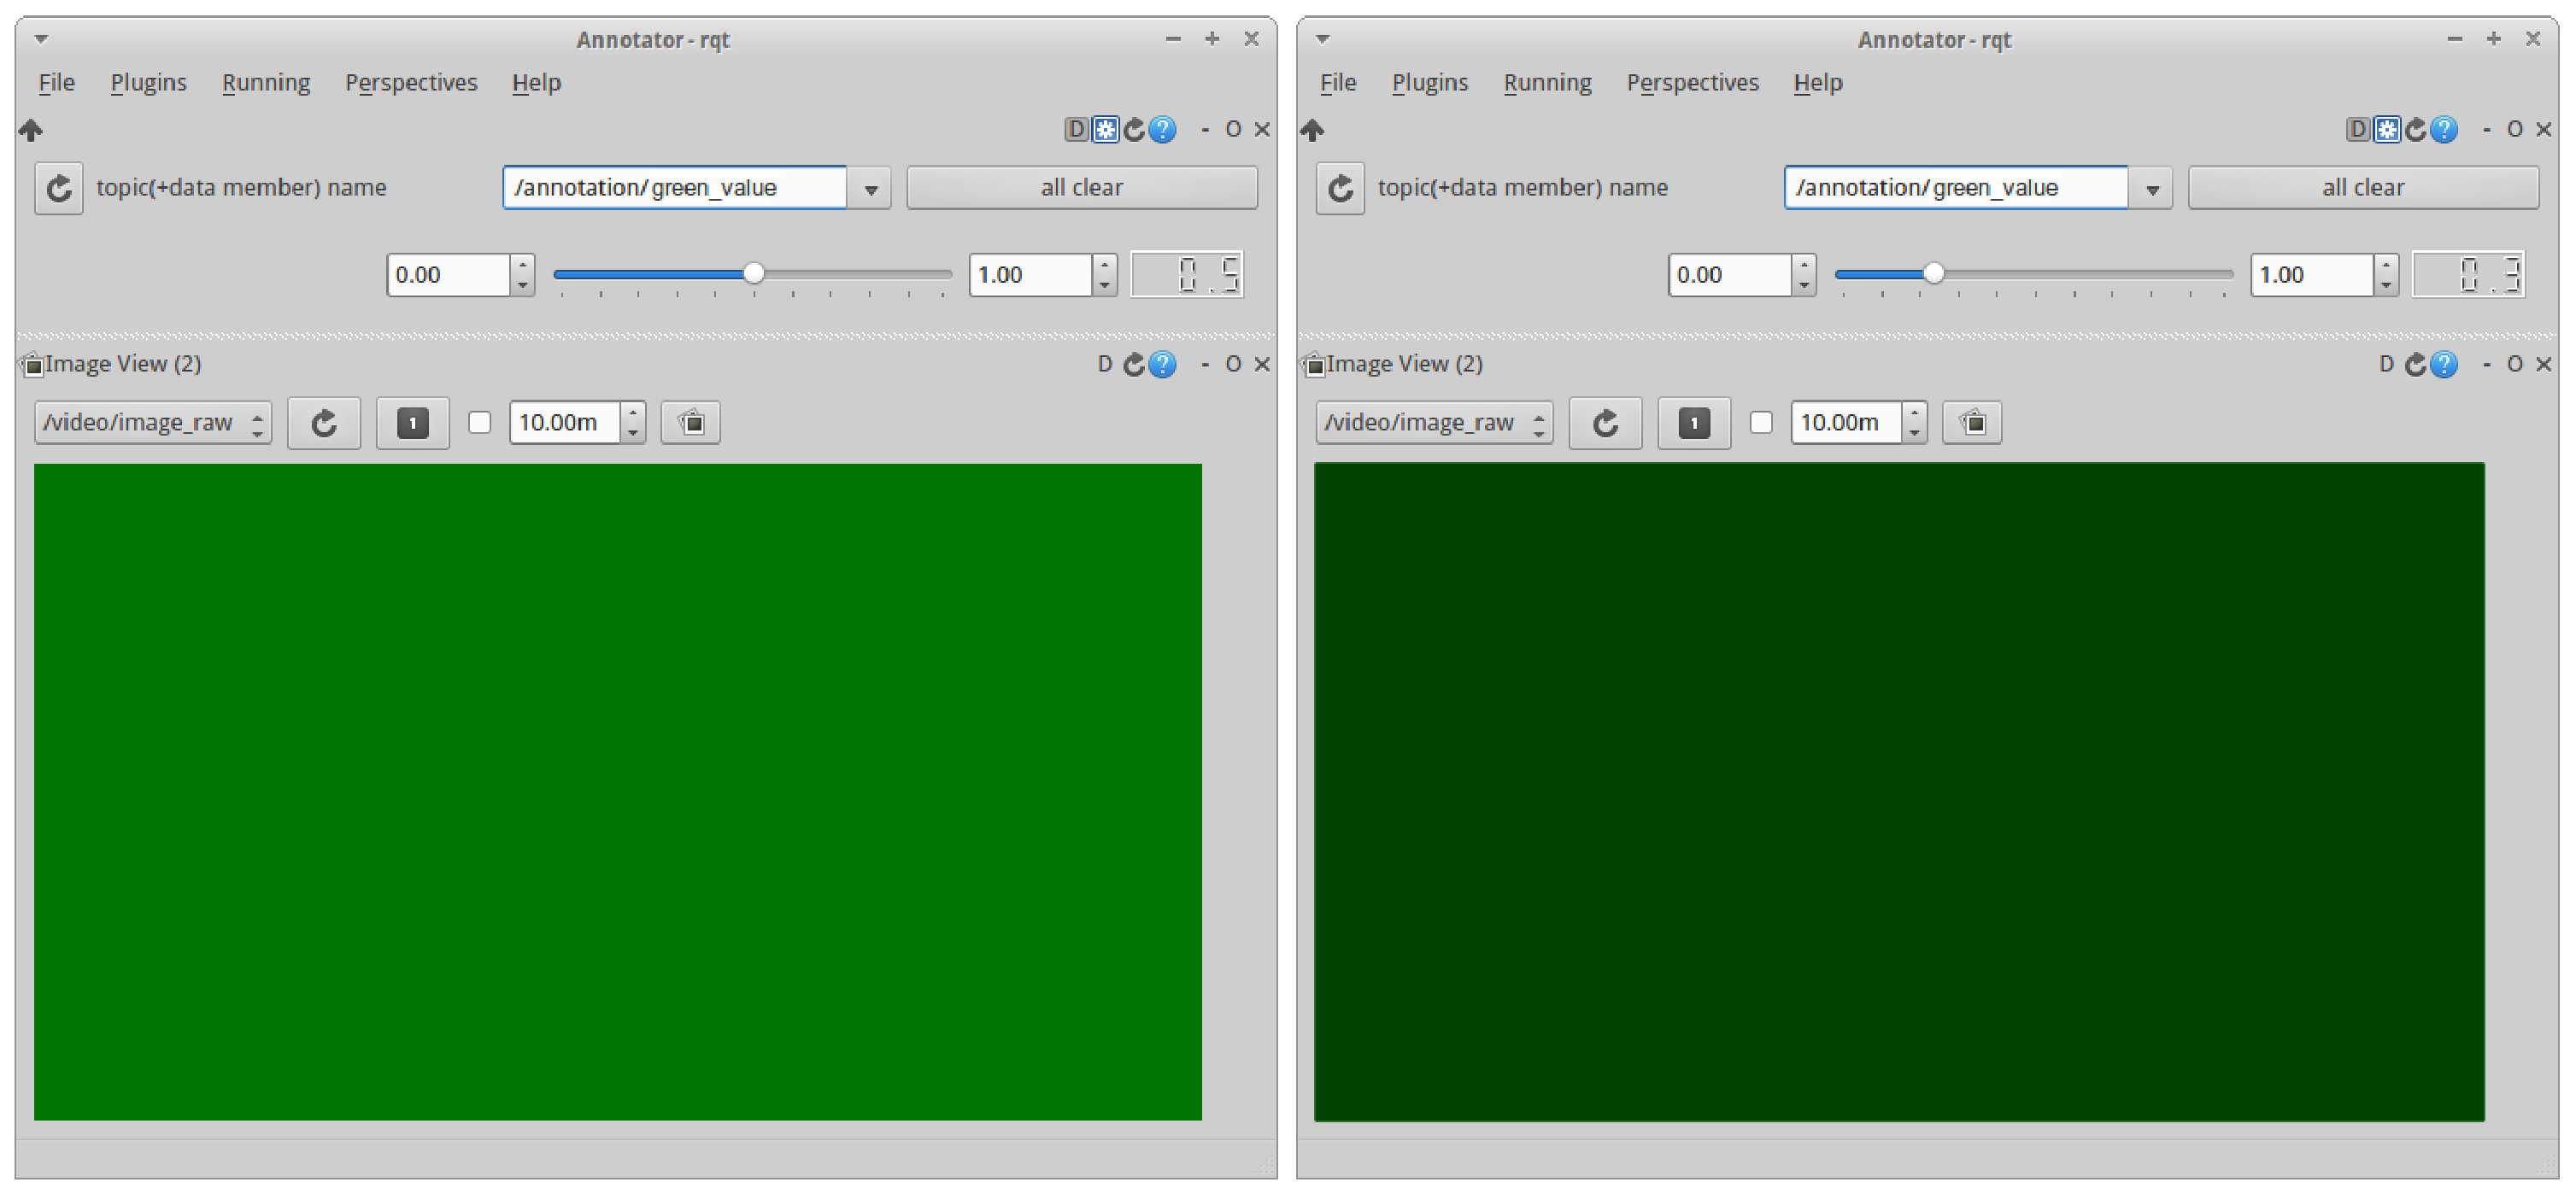
\includegraphics[width=\imagewidth]{images/green_ui.eps}
	\caption{Snapshot of the user interface at different times during the green intensity annotation task.  Annotators only adjusted the slider in sync with changes in the green video.}
	\label{Fig:annotation_ui}
	\end{adjustwidth}
\end{figure}

Fig~\ref{Fig:2} shows a plot of all ten annotations alongside the objective truth for two separate annotation tasks.  Intra-class correlation measures were computed to estimate annotator agreement per the guidelines in \cite{koo2016guideline} and we get 0.97 for each task earning an \textit{excellent} agreement rating according to \cite{cicchetti1994guidelines}.  The ICC values and their 95\% confidence intervals were calculated using the \textit{psych} package version 1.6.9 in R using a mean-rating (k=3), consistency, two-way mixed effects model.

Although the annotator agreement measure is very high and Fig~\ref{Fig:2}c and Fig~\ref{Fig:2}d show that annotators were generally quite good at capturing large-scale changes and trends, they still had difficulties in other areas.  First, most annotators tended to over-shoot the target value when annotating increases or decreases in value over a period of time such as in Fig~\ref{Fig:2}c between 200 and 250 seconds.  This indicates they were perhaps fixated on annotating the rate of change rather than the actual rating.  Notably, annotators were sensitive to and captured the appropriate direction of green intensity changes, but sometimes were also unable to estimate the actual rate of change (see Fig~\ref{Fig:2}c around the 50-second mark).  Secondly, we note that approximately half of the annotators struggled to capture the lack of change in green intensity especially during the 100 to 150-second time interval in Fig~\ref{Fig:2}c.  One possible explanation is that the longer duration of this constant segment gave annotators time to realize their current intensity ratings did not match their perception and then adjust the value to match in spite of what was (not) occurring in the video.  Lastly, we note that similar green intensities were annotated inconsistently over time.  In particular, there was a significant difference in average annotation value per and within an annotator between different time intervals where the green intensity was actually at a constant 0.5 value (see Fig~\ref{Fig:2}a and Fig~\ref{Fig:2}c).

\begin{figure}[t]
    \begin{adjustwidth}{-2.25in}{0in}
	\centering
    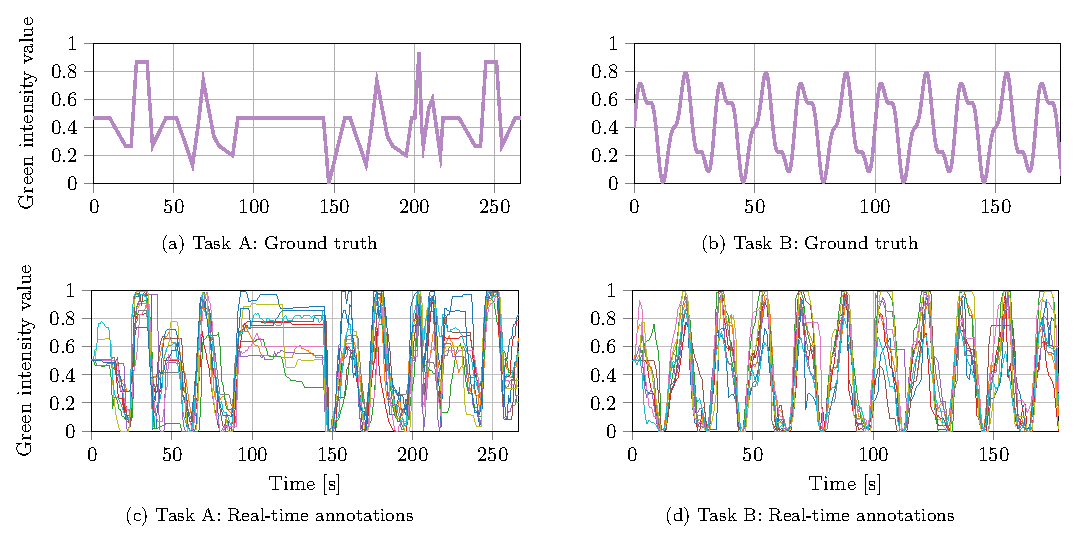
\includegraphics{images/Fig2.eps}
    \vspace{0.2cm}
	\caption{Plots of the objective truths and annotations of green channel intensity from 10 different annotators in two separate tasks.}
	\label{Fig:2}
	\end{adjustwidth}
\end{figure}

This last observation implies that even for this relatively simple annotation task, it is difficult for annotators to accurately capture the trends while preserving self-consistency over time.  Given prior evidence that humans are better at ranking than rating \cite{Yannakakis2011, metallinou2013annotation, yannakakis2015ratings} and our own observations from this study, we assume that in continuous real-time annotation, humans are more focused on and perhaps even better at faithfully capturing trends and less able to accurately assess the true value at any point in time.  In this paper we present a procedure for correcting these rating inconsistencies while preserving the more precise trend annotations.

\section*{Fused Annotation Correction}

We propose a method for warping fused annotations to establish a ground truth signal that has been corrected for various global inconsistencies, artifacts, and errors introduced during the real-time continuous human annotation process.  The method leverages a recurring observation that annotators more successfully capture trends and less accurately represent exact ratings \cite{Yannakakis2011, metallinou2013annotation, yannakakis2015ratings}.  In our approach, additional information in the form of similarity comparisons between unique time segments of the video must be collected from annotators after the continuous annotation task.  We leverage the structure of the fused annotations to identify peaks, valleys, and spans of time where the target construct does not appear to change and we only collect comparisons corresponding to these segments.  This reduces to total amount of additional information that would be required if we were to consider the entire time span.  Further significant reductions to this required supplementary information are discussed in the results section.

Our method is summarized in Fig~\ref{Fig:pipeline}.  The first step fuses the raw annotations together to form a single time series.  This step simply time-aligns and averages all annotations to reduce systemic noise and limit the influence of random annotation artifacts.  In principle, any annotation fusion method could be used at this stage.  Total variation (TV) denoising is then used to approximate the fused signal as a piecewise-constant step function in order to facilitate the identification of segments in time where the target construct does not change noticeably (peaks, valley, and plateaus) and therefore where annotator agreement in rating is likely low.  Constant intervals are extracted from the denoised signal corresponding to time spans where annotators generally agree that the target construct does not noticeably change.  Additional rank information is then procured from annotators to re-evaluate the proper sorting of the these constant intervals with respect to the target construct.  We collect comparison results among unique triplets of these constant intervals and employ an ordinal embedding technique to re-rank them.  Finally, the fused signal is warped piecewise-linearly so the corresponding constant intervals align with the embedding.  These steps and their assumptions are described in detail in the corresponding sections below.

\begin{figure*}[t]
    \begin{adjustwidth}{-2.25in}{0in}
	\centering
	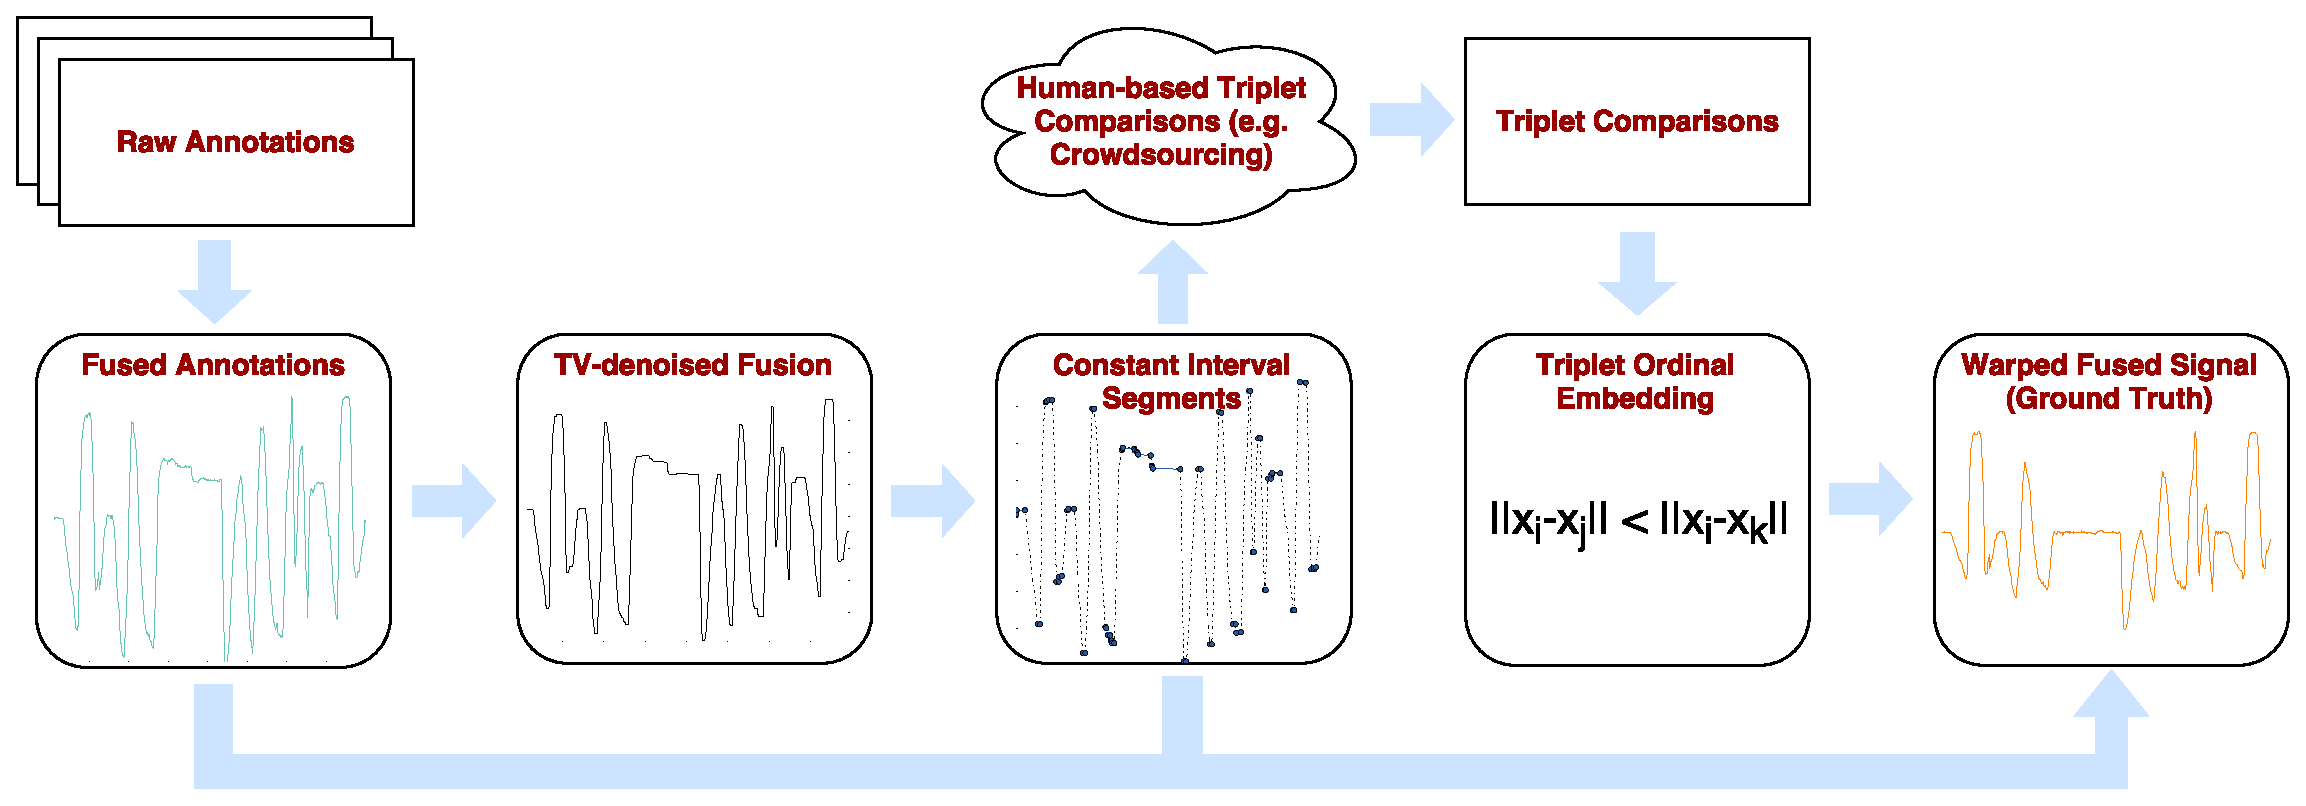
\includegraphics[width=\imagewidth]{images/Fig3.eps}
	\vspace{0.5em}
	\caption{Proposed pipeline for ground truth correction given continuous human annotations.}
	\label{Fig:pipeline}
	\end{adjustwidth}
\end{figure*}
\iffalse
\begin{enumerate}
    \item Lag compensation and averaging
    \item Total variation (TV) denoising
    \item Constant interval extraction
    \item Triplet comparison collection
    \item Ordinal embedding
    \item Fused annotation warping
\end{enumerate}
\fi

\subsection*{Lag Compensation and Averaging (Annotation Fusion)}
The first step involves estimating an appropriate time shift for each annotation signal to align it with the video and compensate for system lag and human reaction time.  Several methods have been proposed for this \cite{DTW2007, CTW2009, andrew2013deep, nicolaou2014dynamic, Mariooryad2015, Ringeval2015, trigeorgis2016deep} and in principle any choice works for this step.  We use a simple per-annotator time shift (\textit{EvalDep}) proposed by Mariooryad et al. \cite{Mariooryad2015}.  This method requires some feature sequences to be extracted from the video for alignment, so we provide the green intensity and its forward difference per frame.  After shifting each annotation by its own lag estimate, we truncate the trailing frames so all annotations are equal length and then average them in time. This lag compensation is not strictly necessary for the success of the proposed method but yields better final results. Fig~\ref{Fig:4}a shows the time-corrected average annotation signal for Task A.

\subsection*{Total Variation Denoising}
Total variation (TV) denoising has been successfully used to remove salt and pepper noise from images while simultaneously preserving signal edges \cite{rudin1992nonlinear}.  In our context, we want to identify the set of peaks and valleys where the annotation rating may be inaccurate, and we also want to find the set of nearly constant regions of the fused annotation signal corresponding to a lack of noticeable change in the target construct.  These regions represent the segments in time when the rating is hypothesized to be least reliable.  Precise extrema and plateau detection in signals is difficult, but in our context we only need to find a compact time interval around each of these regions.  TV denoising is preferable in this case to other smoothing processes both because it approximates the signal as a piecewise-constant step function as is desired, and also because it better preserves the structure.

We use the TFOCS MATLAB library \cite{becker2011templates} to find a new sequence $y$ that approximates a given sequence $x$ by minimizing:
\begin{equation*}
y = \min_{y} \Big[\sum_{t} ||x_t - y_t||_{\ell_2}^2 + \lambda\sum_{t} ||y_{t+1} - y_{t}||_{\ell_1}\Big]
\end{equation*}
The parameter $\lambda$ controls the influence of the temporal variation term and degree to which $y$ is approximately piecewise-constant.  In general this parameter needs to be tuned to produce a desirable sequence.  For this study, we hand-tune $\lambda$ by increasing it by multiples of ten from a very tiny value (e.g. $10^{-8}$) until it first starts appearing piecewise constant instead of ``wavy.''  For both simulated tasks we settle on a value of 0.05.  In principle, this parameter can be automatically selected based on other criteria and heuristics, but we leave this endeavor for future work.  Fig~\ref{Fig:4}b shows an example TV-denoised signal.

\begin{figure*}
    \begin{adjustwidth}{-2.25in}{0in}
	\centering
	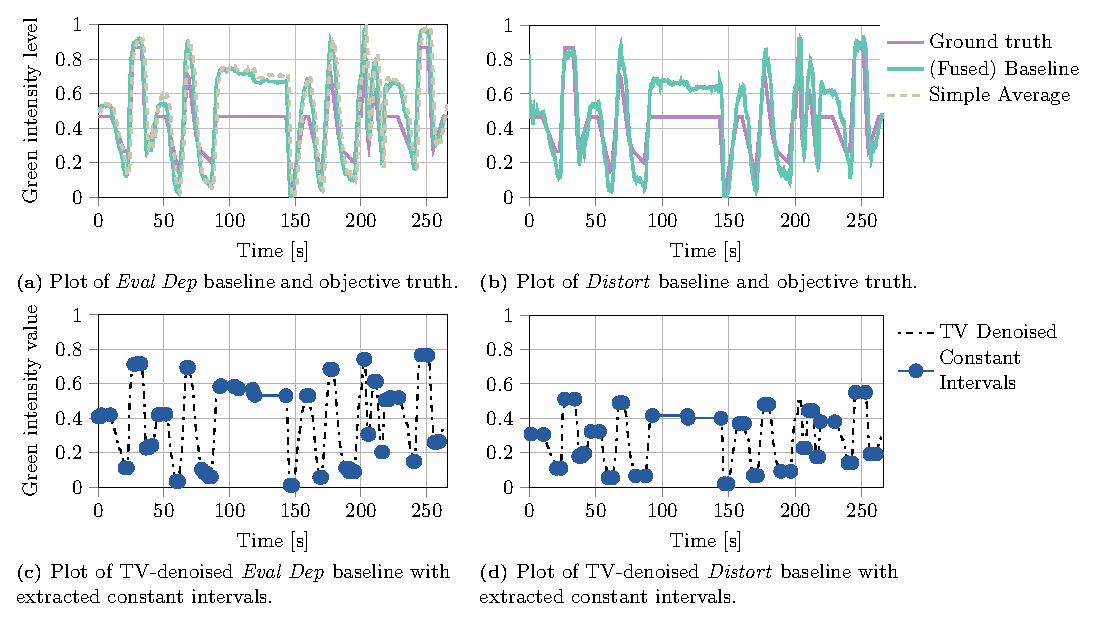
\includegraphics{images/Fig4.eps}
	\vspace{0.5em}
	\caption{Results at intermediate stages of the proposed method pipeline for the \textit{Eval Dep} and \textit{Distort} baselines on Task A.  The \textit{Simple Average} is similar to \textit{Eval Dep} and shown for reference.}
	\label{Fig:4}
	\end{adjustwidth}
\end{figure*}

\subsection*{Constant Interval Extraction}
A simple heuristic is used to extract nearly constant intervals from the TV-denoised signal.  In this step, a scan of the TV-denoised signal is performed and the smallest set of (largest) intervals is found where each interval satisfies two criteria: (1) the total height does not exceed threshold $h$, and (2) the frame length of the interval is at least $T$ frames.  Fig~\ref{Fig:4}b shows the extracted approximately constant intervals for annotation Task A.

The height threshold is chosen to be very small relative to the size of the annotation scale so only very flat regions are considered.  Because TV denoising does well at approximating the signal as a piecewise-constant function, we find this step in the overall procedure is not very sensitive to perturbations of $h$.  The $T$ value is selected to match the duration of the fastest change in the objective truth.  In practice, this parameter could be approximated from the average annotation signal or tuned manually, but should be set no smaller than the equivalent of 0.25 seconds, which is roughly the average human reaction time.  In the future, we hope to obviate these parameters to make this approach more scalable and robust.

\subsection*{Triplet Comparisons}
In this step during an actual experiment, annotators would be asked to compare three extracted video segments corresponding to each unique triplet of constant intervals.  One video segment serves as a reference and the other two as test candidates and the annotator is instructed to select which of the two candidate video segments is most similar to the reference.  For the purpose of assessing the robustness of this approach to missing and conflicting comparison information, we simulate the comparison results using the objective truth as an oracle.  Further analysis of these effects are explored in the results section.

\subsection*{Ordinal Embedding}
Ordinal embedding problems attempt to learn a (typically lower dimension) embedding that preserves a similarity relationship between subsets of data points.  Given a set of inputs $\mathcal{Z} = \{z_1,...,z_n\}$ with each $z \in \mathbb{R}^m$ and a set of similarity relations on 4-tuples from $\mathcal{Z}$ of the form $s(z_i,z_j) < s(z_k,z_l)$ where $\{i,j,k,l\}$ is a 4-subset of $\{1,2,...,n\}$, the goal is to find a set $\mathcal{X} = \{x_1,...,x_n\}$ with each $x \in \mathbb{R}^d$ such that:
\begin{equation*}
||x_i-x_j|| < ||x_k-x_l|| \Longleftrightarrow s(z_i,z_j) < s(z_k,z_l)
\end{equation*}
\noindent
for some norm on $\mathcal{X}$. For our application, we are interested in the case $i=k$ where we have ordinal comparisons in the form of triplets (i.e. sample $i$ is more similar to sample $j$ than $k$).  One reason to prefer this simplification of the general problem is that it reduces the cardinality of the set of all possible comparisons given $\mathcal{Z}$ and thus the amount of additional information we need.  Another rationale is that collecting comparisons over triplets is more intuitive to people and has been studied in prior works \cite{jain2016finite, van2012stochastic}.

Let us briefly explain this natural preference for comparisons over triplets.  Imagine being asked, for example, to assess which two colors are closer to each other: orange and yellow, or green and blue.  The question requires color differences in two different hues to be compared, which is unfair.  Instead imagine yellow is a reference color and the goal is to decide whether orange or green is more similar to it.  The task may still be difficult, but at least the two comparisons are relative to the same object (i.e. it avoids \textit{apples to oranges} comparisons).

A further reduction in the complete number of comparisons would be possible if we consider relationships of the form:
\begin{equation*}
||x_i|| < ||x_k|| \Longleftrightarrow ||z_i|| < ||z_k||
\end{equation*}
for unique index pairs $\{i,k\}$.  This setup supposes that it is possible to directly assign a value to each sample $z$ with respect to the target construct for the purpose of comparing two samples, but this may not always be possible.  In cases where multiple conflicting or ambiguous criteria exist, as in the annotation of smile strength \cite{Gupta2016}, such a scale may not exist or be too unintuitive for human annotators.  So, for generality of this procedure, we choose the triplet comparison approach.

With triplets, the total number of comparisons that can be made when $|\mathcal{Z}|=n$ is $n\binom{n-1}{2} \sim \mathcal{O}(n^3)$.  Fortunately, there is considerable redundancy in the comparison information and only a small fraction is necessary to find an embedding close to the optimal embedding.  Prediction error bounds have already been derived for a slightly different noisy formulation of this triplet embedding problem \cite{jain2016finite}, nonetheless we conjecture that the number of necessary comparisons is $\mathcal{O}(d n\log(n))$ ($d=1$ in our experiment).

In our method, ordinal embedding is used to reorder the constant intervals to make them more self-consistent and rank-aligned with the objective truth.  Several ordinal embedding solvers over triplets have been proposed \cite{agarwal2007generalized, tamuz2011adaptively, van2012stochastic, amid2015multiview}.  We employ the t-stochastic triplet embedding (t-STE) approach \cite{van2012stochastic} because, as the authors highlight, it aggregates similar points and repels dissimilar ones.  We also favor this approach because it prefers the simpler explanation that two points in the embedding are identical when no evidence suggests otherwise (Occam's Razor principle).  Fig~\ref{Fig:warp_evaldep} shows the embedding results for the extracted constant intervals that have been rescaled to the proper $[0,1]$ range and computed using a complete set of triplet comparisons from the oracle.  Note that the embedding only preserves the relative similarity relationships, so the embedding is expected to be off by a (unknown) monotonic transformation of the objective truth.

\begin{figure*}
    \begin{adjustwidth}{-2.25in}{0in}
	\centering
    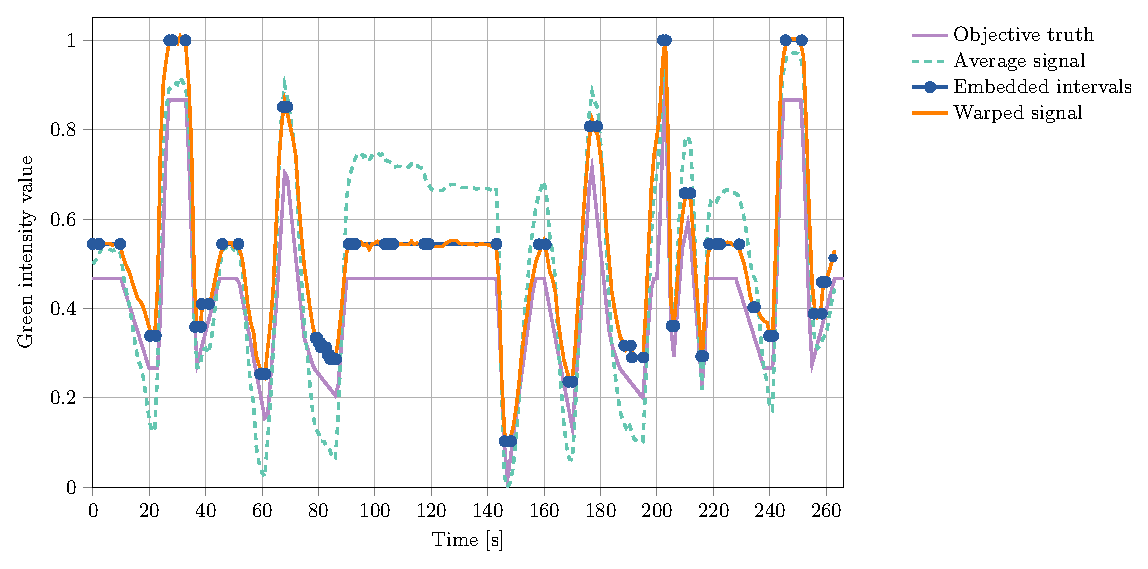
\includegraphics{images/Fig6.eps}
    \vspace{0.5em}
	\caption{Plot of the objective truth signal, time-shifted average annotation signal, warped signal, and the 1-D embedding for extracted constant intervals for Task A.  The spatially warped signal better approximates the structure of the objective truth and also achieves greater self-consistency over the entire annotation duration.}
	\label{Fig:warp_evaldep}
	\end{adjustwidth}
\end{figure*}

\subsection*{Spatial Warping}

In the final step, the fused annotation is spatially warped to rectify inconsistencies using the ordinal embedding results.  Within the time frame of each interval, the fused annotation is shifted so its average over the interval is equal to its corresponding embedding value.  The fused annotation between each constant interval is offset and linearly scaled to align with its neighboring repositioned constant intervals.  We select a linear inter-interval warping function because it avoids distorting the signal.  A formal definition is given in Eqs~(\ref{eqn:interval_difference},\ref{eqn:warp}) in Fig~\ref{Fig:equations}.  Fig~\ref{Fig:warp_evaldep} shows the results after applying this warping technique.

\begin{figure*}[!t]
\begin{adjustwidth}{-2.25in}{0in}
\normalsize
%\setcounter{MYtempeqncnt}{\value{equation}}
\setcounter{equation}{0}
\begin{eqnarray}
\label{eqn:interval_sequence}
\mathcal{I}_i &=&
\begin{cases}
\{t : \min(\mathcal{C}_i) \leq t \leq \max(\mathcal{C}_i)\} & i \in \{1,2,...,|C|\} \\
\{0\} & i = 0 \\
\{T\} & i = |C|+1
\end{cases}\\
\label{eqn:interval_difference}
S_i &=&
\begin{cases}
\mathcal{E}_i - \frac{1}{|\mathcal{I}_i|}\sum\limits_{t\in\mathcal{I}_i} y_t & i \in \{1,2,...,|C|\} \\
0 & \text{else}
\end{cases}\\
\label{eqn:warp}
y_t' &=&
\begin{cases}
y_t + S_i & \exists \mathcal{I}_i : t \in \mathcal{I}_i \\
y_t + \Big(\frac{y_t-y_a}{y_b-y_a}\Big)\mathcal{S}_{i+1} + \Big(\frac{y_b-y_t}{y_b-y_a}\Big)\mathcal{S}_i & \exists i : a \leq t \leq b, a = \max(\mathcal{I}_i), b = \min(\mathcal{I}_{i+1})
\end{cases}
\end{eqnarray}
%\setcounter{equation}{\value{MYtempeqncnt}}
% IEEE uses as a separator
\hrulefill
% The spacer can be tweaked to stop underfull vboxes.
\vspace*{4pt}
\caption{Equations for our proposed spatial warping method.  Let $t \in \{1,2,...,T\}$ be a time index, $y_t$ denote the fused annotation signal, $y'_t$ denote the warped signal value, and let $\mathcal{C}$ be the ordered sequence of non-overlapping time intervals corresponding to the extracted constant intervals.  We define $\mathcal{E}$ as the sequence of embedding values in $\mathbb{R}^d$ corresponding to the time interval sequence $\mathcal{C}$.  The sequence $\mathcal{I}$ is used instead of $\mathcal{C}$ to handle edge cases.  For notational simplicity, we also introduce a new sequence $S$ whose $i$'th element is the difference between interval $i$'s average value and the corresponding embedding value.}
\label{Fig:equations}
\end{adjustwidth}
\end{figure*}

\section*{Results}
Using the \textit{Eval Dep} method from Mariooryad et al. \cite{Mariooryad2015}, we estimate the lag for each annotator and find that the average lag is approximately 1.6 seconds.  In the constant interval extraction stage, we use a height threshold $h=0.003$ and a minimum frame count threshold $T=17$ (recall the videos are 30Hz).  We choose $h$ to be quite small relative to the annotation scale and find that for well-TV-denoised signals the method is not very sensitive to this parameter.  The $T$ parameter was simply selected to be the smallest value greater than ten (average human reaction time) that produced a manageable number of intervals.

Table \ref{tab:results} shows various agreement measures for the objective truth and prior established annotation fusion approaches that are intended to produce ground truth estimates.

\setlength\tabcolsep{1pt}
\setlength\extrarowheight{1pt}
\begin{table}[ht!]
\caption{\label{tab:results} Agreement measures for baseline and proposed warped fused annotation approaches}
\centering
\begin{tabular}{ cccccc } 
 \Xhline{2\arrayrulewidth}
 \textbf{Task} & \textbf{Signal Type} & \textbf{Pearson} & \textbf{Spearman} & \textbf{Kendall's} & \textbf{NMI} \\
  & & & & \textbf{Tau} & \\
 \Xhline{2\arrayrulewidth}
 \multirow{6}{*}{\textbf{A}} & Simple Average & 0.775 & 0.795 & 0.636 & 0.302 \\ 
 & Warped Average & 0.811$^\dagger$ & 0.738 & 0.584 & 0.307 \\
 \cline{2-6}
 & Distort$^{*}$ & 0.809 & 0.834 & 0.676 & 0.793 \\
 & Warped Distort & 0.888$^\dagger$ & 0.839 & 0.695 & 0.794 \\
 \cline{2-6}
 & EvalDep$^{**}$ Average & 0.906 & 0.946 & 0.830 & 0.484 \\
 & Warped EvalDep & 0.967$^\dagger$ & 0.939 & 0.835 & 0.562 \\
 \Xhline{2\arrayrulewidth}
 \multirow{6}{*}{\textbf{B}} & Simple Average & 0.950 & 0.948 & 0.804 & 0.772 \\ 
 & Warped Average & 0.964$^\dagger$ & 0.960 & 0.828 & 0.859 \\
 \cline{2-6}
 & Distort$^{*}$  & 0.967 & 0.966 & 0.848 & 0.955 \\
 & Warped Distort  & 0.960 & 0.962 & 0.842 & 0.957 \\
 \cline{2-6}
 & EvalDep$^{**}$ Average  & 0.969 & 0.969 & 0.855 & 0.774 \\
 & Warped EvalDep  & 0.988$^\dagger$ & 0.987 & 0.906 & 0.862 \\
 \Xhline{2\arrayrulewidth}
\end{tabular}
\vspace*{4pt} \\
{\footnotesize All warped results use a complete set of ordinal comparisons from the oracle. NMI = normalized mutual information.  \\ $^\dagger$ - significant improvement ($p<0.005$, using a Fisher z-transform) of the warped methods over the respective signal \\ $^{*}$ - method from \cite{Gupta2016} \\ $^{**}$ - method from \cite{Mariooryad2015}}
\end{table}
Three baseline annotation fusions are shown, one is an average (\textit{Simple Average}) of the expert annotations, one is the maximum likelihood estimation (\textit{Distort}) from a per-annotator distortion model \cite{Gupta2016}, and the last is a time-aligned average (\textit{Eval Dep}) using evaluator-dependent time shifts \cite{Mariooryad2015}.  Our rank-based warping method is applied to each baseline using a full set of triplet comparisons from the oracle.  In all cases except for one, the warping method achieves significantly better results ($p<0.005$) when agreement is measured using Pearson correlation or normalized mutual information.  In the one outlier case, the \textit{Distort} model already approximates the objective truth extremely well because the true signal for Task B is very smooth.  In this case, the proposed warping method does not diminish the correlation considerably.

Although one would na\"ively expect the proposed rank-based signal warping procedure to improve rank-based correlation metrics, Spearman and Kendal's Tau correlations slightly decrease in some cases.  This is primarily due to frame-level rank disagreements over the warped constant intervals, rather than disagreements at a large scale due to the ordinal embedding.  The same decrease in rank-based correlation can occur when any non-injective function is piecewise linearly warped and thus is not unique to the proposed method.

We would like to be able to compare the mean squared error between the warped signal and the objective truth, but the optimal embedding results used to warp the signal are indistinguishable under monotonic transformations over the embedding values.  This means the warped signal will only be structurally similar to the objective truth, but not necessarily identical.  If this disparity is severe enough, the relationship between the objective truth and warped signal may be very non-linear suggesting that even Pearson correlation may decrease.  Thus we postulate that the best measure of success is self-consistency of the resulting corrected fused signal because it further minimizes the amount of variance that needs to be explained by any learned model.

Lastly, we briefly address the robustness of the proposed warping method to incomplete triplet comparisons. Even for modest numbers of constant intervals, the number of triplets required for a complete set grows cubicly.  Due to the large amount of redundancy in the triplet comparisons, only a small fraction is necessary for the warping method to approximate the objective truth well.  Fig~\ref{Fig:warp_correlation_robustness} shows a plot of the performance of this spatial warping approach for both incomplete triplet comparisons and partially adversarial comparisons.  In Task A, there are 40 extracted intervals and thus 29,640 possible comparisons.  Assuming a five percent triplet comparison error rate, significant improvement over the best tested baseline method is achieved with only two percent, or about 600, randomly selected triplet comparisons.

\begin{figure}[t]
    \begin{adjustwidth}{-2.25in}{0in}
	\centering
    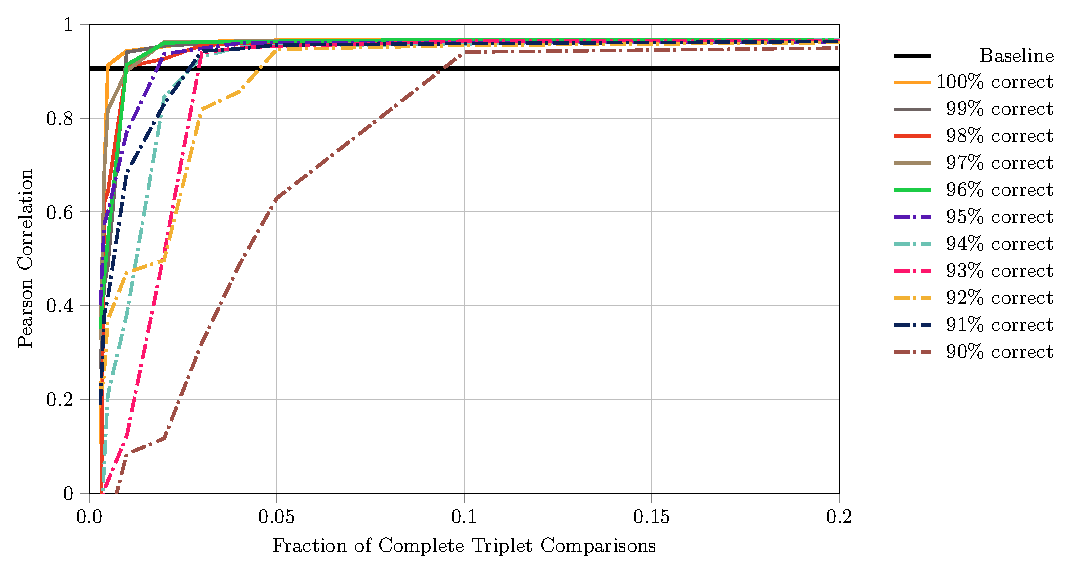
\includegraphics{images/Fig7.eps}
	\caption{Plot showing Pearson correlation of the warped annotation from Task A and the fusion from \cite{Mariooryad2015} for different percentages of the total number of possible triplet comparisons.  Several plots are shown for varying levels of average annotation accuracy.  A high correlation is possible with a small fraction of the triplets due to large amounts of redundancy in the comparisons. The black line represents the best baseline method's correlation.}
	\label{Fig:warp_correlation_robustness}
	\end{adjustwidth}
\end{figure}

\section*{Future Work}
There are several compelling research directions for expanding on this work which we aim to address in the future.  The total variation denoising procedure requires careful selection of an unintuitive tunable constant to achieve desirable results.  Consideration of other problem constraints, such as the budget of financial resources available for annotation or the required accuracy on predictions from the resulting ground truth, could be used to find a sensible value for this parameter.  The subsequent constant interval extraction step also has two parameters that could be chosen automatically from the data given some additional heuristics or constraints.  Further analysis of this method's ability to produce accurate ground truth estimates for more complex continuous annotation tasks, like 2-D dimensional affect, is another exciting avenue.  Larger reductions in the number of required triplet comparisons may also be possible using adaptive sparse sampling techniques to pick the next most informative triplets for comparison and stochastic transitivity to infer some triplet comparisons from the fused annotation automatically.

\section*{Conclusion}
In this paper we propose a novel method for extending continuous real-time human annotation fusion approaches to generate a more accurate ground truth.  We leverage the natural ability of annotators to provide accurate similarity comparisons and propose a procedure for warping the fused annotation to better align with the target construct.  We test our approach in a mechanically simple but perceptually difficult annotation experiment where an objective truth is known and show that our approach yields a signal significantly more correlated with the objective truth in spite of the presence of several annotation artifacts.  We hope this method finds utility as a means for establishing a more accurate ground truth in hidden state problems where no objective truth is available \textit{a priori}.

All data and code used for this study can be found at: \href{https://github.com/brandon-m-booth/2016_continuous_annotations}{https://github.com/brandon-m-booth/2016\_continuous\_annotations}.

\section*{Acknowledgments}

\bibliographystyle{plos2015}
\bibliography{sample}

% \begin{thebibliography}
% \end{thebibliography}

\iffalse
\begin{table}[ht!]
\centering
\begin{tabularx}{\textwidth}{ |K{1in}|C|C|C|C|C|C|C|C| } 
 \hline
 Annotation Artifact Sources & \multicolumn{8}{|c|}{Approximate Effect} \\
 \hline
 & Time shift & Mean bias & Variance bias & Local decoherence & Global decoherence & Decreased coherence & Improved coherence & Negative correlation \\
 \hline
 Human Reaction Lag & \X & & & & & & & \\ \hline
 System Input Processing Lag & \X & & & & & & & \\ \hline
 Input Errors & & & & \X & & & & \\ \hline
 Initial Input State & & \X & & & & & &\\ \hline
 Acclimation to Task & & & & & & & \X & \\ \hline
 Fatigue & & & & & & \X & & \\ \hline
 Iconic/Echoic memory duration & & & & & \X & & & \\ \hline
 Recalling similar annotation event & & & & \X & & & & \\ \hline
 Perception bias & & \X & \X & & & & & \\ \hline
 Experience bias & & \X & \X & & & & & \\ \hline
 Distractions & & & & \X & & & & \\ \hline
 Preoccupations / Mood & \X & \X & \X & \X & \X & & & \\ \hline
 Context bias & & \X & \X & \X & \X & & & \\ \hline
 Adversarial annotation & & \X & \X & \X & \X & & & \X \\ \hline
 Cognitive workload & \X & & & \X & & & & \\
 \hline
\end{tabularx}
\caption{Possible sources of annotation artifacts from a real-time continuous annotation process and the effect each has on the annotation signal.}
\label{tab:results}
\end{table}
\fi

\end{document}